\section{Méthode}

\subsection{Dataset}

Nous utilisons le dataset fournit pour la tâche 3 de l’édition 2009 de DEFT.
Il s'agit d'un corpus multilingue de débats parlementaires européens. Chaque intervention
parlementaire est classée en fonction du parti \footnote {ELDR, PPE-DE, PSE, GUE-NGL et Verts-ALE}
du locuteur et présente dans le corpus dans 3 langues : anglais, français et italien.\\
Au moment de faire des statistiques descriptives, nous nous sommes rendus comptes 
que le corpus présentait des doublons, et ce majoritairement dans la partition test.
\begin{figure}[ht]
    \centering
    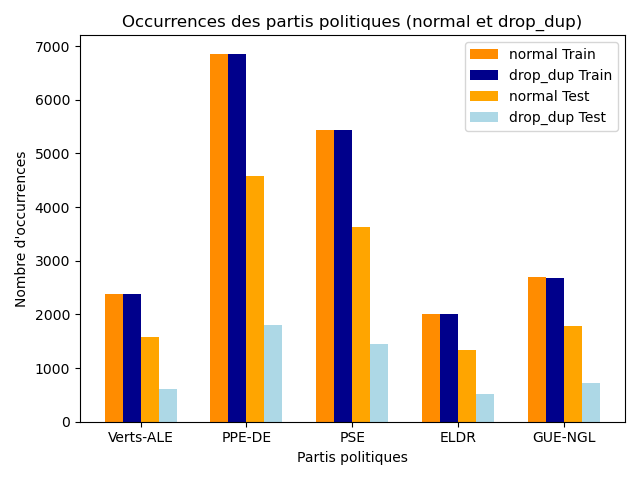
\includegraphics[width=\columnwidth]{../stats/occurences_orig_vs_drop_dup_par_cat.png}
    \caption{Nombre d'interventions par parti par partition test/train, dans le corpus original et dans la version sans doublons}
    \label{fig:barplot_dataset}
\end{figure}

Après suppression des doublons, la partition prévue (40/60) est changée : elle est 
maintenant de 20/80\footnote{ 0.79 pour le train et 0.21 pour le test}.
Nous avons envisagé de réimplémenter le partitionnement prévu, mais avons renoncé pour deux raisons : 
refaire le partitionnement nous éloigne, encore, du corpus initial, et les 
résultats de quelques modèles sur un corpus repartitionné étaient proches des résultats 
sur cette partition 20/80.
Par ailleurs, la répartition des classes est déséquilibrée : les classes PPE-DE et PSE sont plus grandes et forment à elles deux 63,5 \% du corpus. Ceci devra être 
pris en compte dans le prétraitement.\footnote{la figure correspond au train, mais la répartition est sensiblement la même dans le test}

\begin{table}[ht]
    \centering
\begin{tabular}{|l|l|l|}
\hline
Statistique & Train & Test \\ \hline
Moyenne & 3871.4 & 1021.2 \\ \hline
STD & 2149.1 & 569.7 \\ \hline
Min & 2005.0 & 525.0 \\ \hline
1er quartile & 2376.0 & 615.0 \\ \hline
Médiane & 2687.0 & 715.0\\ \hline
3eme quartile & 5431.0 & 1448.0\\ \hline
Max & 6858.0 & 1803.0\\ \hline
\end{tabular}
\caption{Nombre d'intervention des partis par partition}
\label{tab:stats_dataset}
\end{table}

\begin{figure}[ht]
    \centering
    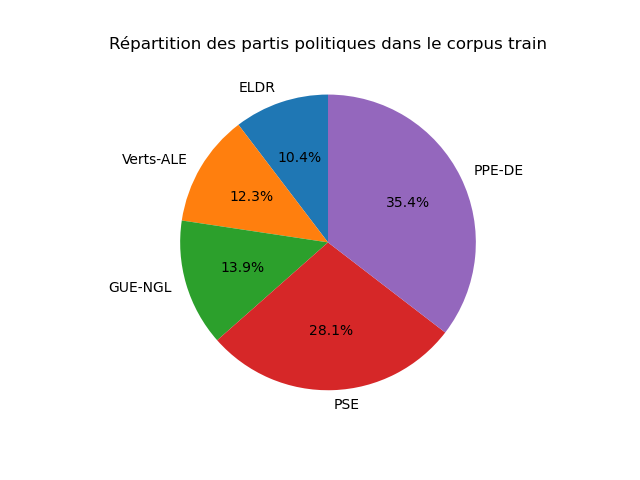
\includegraphics[width=\columnwidth]{../stats/occurences_par_partis_train_camember.png}
    \caption{Répartition des interventions par parti dans la partition train sans doublons}
    \label{fig:camember_dataset}
\end{figure}
\subsection{Prétraitements}
Le texte des interventions a été soumis à un prétraitement simple :\\
\indent(1) Suppresion de la ponctuation\\
\indent(2) Unification de la casse en minuscules\\
\indent(3) Tokenisation\footnote {Une lemmatisation avec la bibliothèque SpaCy a été envisagée,
mais ce corpus multilingue aurait nécessité le chargement de 3 modèles linguistiques
différents et ralongé d'autant le temps de traitement}
\\
Pour résoudre le problème de déséquilibre des classes, nous avons opté pour le 
\textit{downsampling} afin d'obtenir des classes relativement équilibrées,
en utilisant la fonction \textit{resample} de la bibliothèque Sckit-learn. Après \textit{downsampling},
les classes PPE-DE et PSE ne représentent plus que 43\% du corpus, ayant chacune été ramenée autour de 21,5\% du corpus

\begin{table}[ht]
    \centering
\begin{tabular}{|l|l|l|}
\hline
Parti & Train & Test\\ \hline
ELDR & 2531 (16,1\%) & 525 (16,2\%) \\ \hline
PPE-DE & 3402 (21,63\%) & 715 (22\%) \\ \hline
GUE-NGL & 3402 (21,63\%) & 687 (21,2\%) \\ \hline
PSE & 3402 (21,63\%) & 693 (21,4\%) \\ \hline
Verts-ALE & 2990 (19\%) & 614 (19\%)\\ \hline
Total & 15727 & 3235\\ \hline
\end{tabular}
\caption{Nombre d'intervention par parti par partition pour une langue après \textit{downsampling}, example de l'italien}
\label{tab:stats_downsampled}
\end{table}


\subsection{Les différents embeddings testés}
Nous avons choisi dans notre étude de comparer les résultats obtenus sur une tâche 
de classification en utilisant 3 techniques de vectorisation différentes.\\
\indent La vectorisation TF-IDF\footnote{Implémentée avec la fonction tfidfvectorizer de Scikit-learn} bibliothèque (\textit{Term Frequency-Inverse Document Frequency})
est la méthode la plus "ancienne" que nous présentons. Elle se base sur une mécanique de comptage des mots:
la fréquence d'apparition de chaque mot dans un document est divisée par sa fréquence d'apparition dans le corpus,
permettant de donner plus d'importance aux mots significatifs dans leurs documents d'apparition.\\
\indent La vectorisation Doc2Vec une une vectorisation de document plutot que de mot. Ces vecteurs sont
l'ouput d'un réseau de neurones et nécessite donc une phrase d'entrainement. Pour cette étude,
nous avons choisi de générer des vecteur Doc2Vec à 100 dimensions\footnote{il serait possible de faire plus, mais nous essayions de ne pas saturer nos machines}
avec une fenêtre glissante de 5 mots et d'ignorer les mots n'apparaissant pas au moins 3 fois.\\
\indent La vectorisation avec BERT. Ce modèle basé sur les réseaux de neurones s'appuie sur une 
architecture transformer et nécessite également une phase d'entrainement. Contrairement à
Doc2Vec, elle renvoie des vecteurs de mots, et utilise un mécanisme d'attention lors de
la génération des vecteurs, lui permettant de prendre en compte l'importance d'un mot en fonction du contexte local dans
lequel in apparait.





